\chapter{Optics Lab: Introduction}

\chapterprecis{Optics Practicum 2}

\makeoddhead{myheadings}{\emph{Optics Lab: Introduction}}{}{\thepage}
\makeevenhead{myheadings}{\thepage}{}{\emph{Optics Practicum 2}}

\section*{Introduction}

In our readings from \emph{The Principles of Quantum Mechanics}, Dirac proposes thought experiments to spell out some of the peculiar logic of quantum theory. We will perform versions of those experiments ourselves in the quantum optics laboratory in the basement of Mellon Hall. All will employ the same basic suite of equipment, which includes some devices like those used in the polarization practicum---lasers, photodiode detectors, and a variety of polarizers and waveplates---as well as some new elements: a high-speed coincidence detector and individual photon counters, a computer interface to display results of experiments, beam-splitters and mirrors to direct light, and perhaps most consequentially, a down-conversion crystal, an optical element so called because it converts some portion of a beam of light of a higher frequency to a pair of beams of light of lower frequencies (in our setup, from the 405 nm laser to a pair of beams at wavelengths near 810 nm).

What we will do in this practicum is not one of Dirac's thought experiments, but they all depend on something like it, namely, the ability to grapple with light as quanta. All the elements of our apparatus help us to do this, but perhaps none so much as the down-conversion crystal and the detectors. The crystal works for reasons it takes advanced quantum mechanics to explain, and so to explain its action is beyond our scope, but at least some of its practical effects are understandable, and in a way it resembles the Iceland spar in exhibiting birefringence. In our final practicum, we will depend on a distinctly non-classical effect of an arrangement of two such crystals. As stated above, the crystal splits a small portion of a beam of laser light into two dimmer beams---\emph{much} dimmer---so dim, in fact, that our powerfully amplified photodetectors and fast coincidence counters can register individual photons (though they do not register every photon).

In this practicum, in order to familiarize ourselves with the equipment for later practica, we will use it to demonstrate the particle-like character of light, by sending light through a beam-splitter and closely measuring the light that emerges. The beam-splitter exploits the partial reflection that occurs at the interface between two media to send incident light into two different directions or to combine incident beams into a single beam (see Fig.\ 1). The phenomenon of partial reflection is familiar (e.g., in any window pane), but predicting how light composed of photons will behave in the beam-splitter takes a little bit of thought. A naive first thought, preserving both the phenomenon of partial reflection and the theory of light quanta, might be that each photon of light striking a partially reflecting surface is split into two photons, one reflected, one transmitted. But if you look at a partial reflection, think about the conservation of energy and the relation of energy and wavelength, and realize that the colors of the reflected image are the same as the original, and not some longer-wavelength colors, you can see that this can't be what is happening.

%%%%%%%%%%%%%%%

\begin{figure}[h] 
  \begin{center}
    \captionsetup{width=.75\textwidth}
    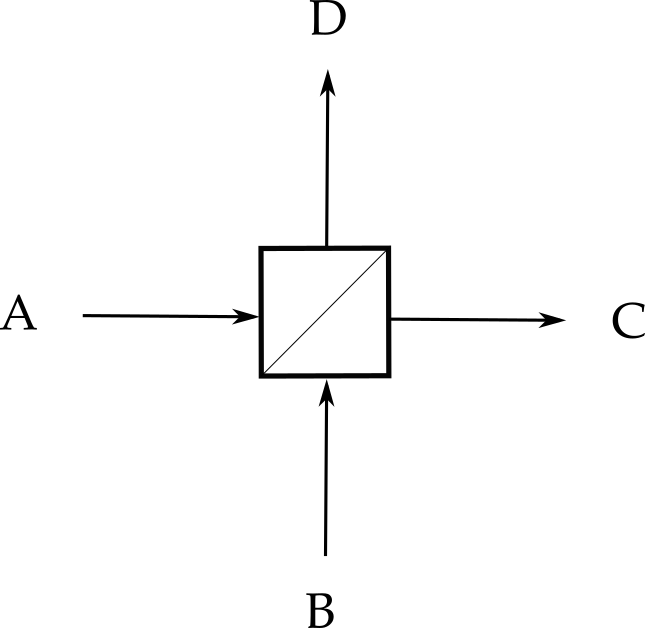
\includegraphics[width=2.15in,height=2.09333in]{images/13_optics-lab/beam-splitter.png}
    \caption*{Figure 1: Light enters the beam-splitter from $A$ or $B$, and exits to either $C$ or $D$.}
  \end{center}
\end{figure}


A second thought, perfectly adequate and effectively a version of the theory we will test, preserves the integrity of the photon in the face of the phenomenon of partial reflection, claiming only that \emph{some photons are reflected, some are transmitted}. This is compatible with many different accounts of what determines which photons go which way. Despite being broadly indeterminate in this way, it is definite enough to have one important testable prediction: a single photon leaving the beam-splitter must emerge from one or another side, and not both. If the beam is dim enough and the counters sensitive enough and the coincidence detectors fast enough (and we have good reasons to believe they all are), we can test this prediction. In Figure 2, if the laser light enters the beam-splitter and detectors are placed at $B$ and $B'$, we should (almost) never find a ``coincidence''---i.e., a count occurring within the time window of our coincidence detector, on the order of several nanoseconds---between firings of the detectors at $B$ and $B'$. (More on the detector at $A$ in the description of the analysis of results below. More, too, on that ``never.'')

%%%%%%%%%%

\begin{figure}[h] 
  \begin{center}
      \captionsetup{width=.75\textwidth}
    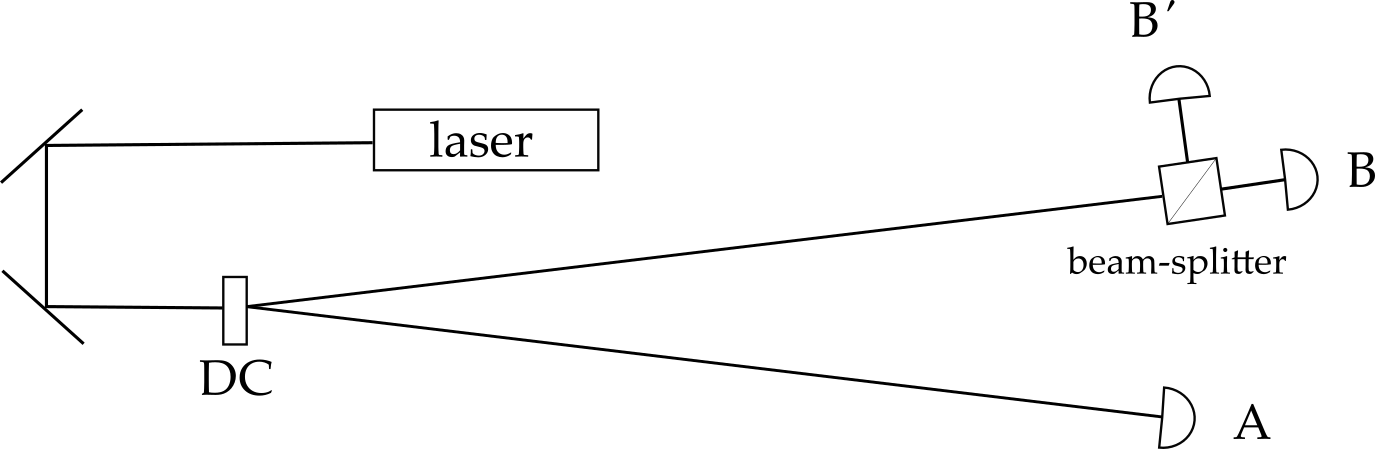
\includegraphics[width=4.58333in,height=1.49667in]{images/13_optics-lab/apparatus.png}
    \caption*{Figure 2: Light from one beam leaving the down-conversion crystal ($DC$) enters the beam-splitter, which either transmits it to detector $B$ or reflects it to detector $B'$.}
  \end{center}
\end{figure}



While our authors often frame their thought experiments in terms of the behavior of a single photon or a single electron, we must recall considerations like Heisenberg's and Dirac's about the inevitability of disturbing single particles with any interaction leading to measurement. We cannot usefully observe a single photon "in flight," as it were, to confirm that it behaves as our theory says it must. More than that, because of the extreme delicacy (and therefore lack of accuracy) of the measurements we are trying to take (registering \emph{single} photons!), we cannot rely on the results of a single measurement. We will instead aggregate the results of thousands, tens of thousands, and even millions of measurements.

The sort of question to which such results can provide an answer, then, is statistical in nature: according to the theories we are trying to test, what results are possible? And in this particular case, how well \emph{correlated} are the individual detections of photons from the the two outputs of the beam-splitter? If light is composed of photons and our instruments are perfect, there should be near-perfect \emph{anti-correlation} between the two detectors: if one fires in a given 4 ns window, the other should not, except in the extremly unlikely instance that two photons happen to be coming through the beam-splitter during that same window of time. Let's make the measure of correlation and anti-correlation more quantitative.

If $P(BB')$ is the probability of both detectors firing within our detection window, and $P(B)$ and $P(B')$ are the probabilities of detector $B$ or $B'$ firing within that time, then a measure of the correlation of the two detectors firing at the same time (which we will call $g$) is

\[g = \frac{P(BB^\prime)}{P(B) \cdot P(B^\prime)} \; . \]


%%%%%%%  explain why calculated this way  %%%%%%%%%%%%%

Again, if light is composed of photons is thus going either one way or the other through the beam-splitter, $P(BB')$ should be zero, with the result that $g$ is zero.  If not, then the firing of detector $B$ may be completely unrelated to the firing of detector $B'$.  Both detectors would simply fire randomly at some average rate.  Therefore, on this latter hypothesis, the probability that both $B$ and $B'$ will fire in a given time is simply the product of the probability that $B$ will fire and the probability that $B'$ will fire; that is, $P(BB') = P(B)\cdot P(B')$. If this is the case, the correlation $g$, which compares those two probabilities, will equal one.  There is no classical theory of the behavior of light that predicts correlations less than one. Our competing theories thus make distinct predictions about the outcome of the experiment.

Our practicum will involve collecting data that will give us a measurement for $g$.  If $g<1$, you will have shown that the classical account is inadequate to explain the results, and this presence of anti-correlation is consistent with the theory that light is composed of photons.  (A $g$ equal to zero is ideal.  Various factors, including the sensitivity of our instruments and the difficulty of excluding every photon except the ones from our light source, ensure that our measurement of $g$ will never be zero.  Anything less than one, however, is not explainable in terms of classical mechanics and is therefore taken as consistent with the quantum theory of light.)


%%%%%%%%%%%%%%%%%%%%%%%
%%% BEGIN HERE
%%%%%%%%%%%%%%%%%%%%%%%%
% waiting for answers
% to queries about eqpmt
%%%%%%%%%%%%%%%%%%%%%%%%`

\section*{Data Collection}

The extreme sensitivity of our instruments makes it important to control the light that is 
reaching them as stringently as possible, so we can be sure the conclusions we draw about the nature of light from our experiments are well-founded. In the present case, that means counting detections at our B and B' detectors \emph{only when light is detected at A, also.} As a practical matter, you can take data without this additional restriction, too, and compare results. Including coincidences with counts at A, our formula for $g$ must change:

\[g = \frac{P(ABB^\prime)}{P(AB) \cdot P(AB^\prime)} \; .\]


To acquire numbers for our probabilities, we will take counts over a five second time period.  The number of counts in each detector is proportional to the probability of light hitting that detector.  We will normalize everything to the counts at detector A, expressing all our counts as fractions of the total counts at A.  We will denote the number of counts at detector A as N(A), etc., so that

\[P(ABB^\prime) = \frac{N(ABB^\prime)}{N(A)} \]


 \[P(AB) = \frac{N(AB)}{N(A)} \]

\[P(AB^\prime) = \frac{N(AB^\prime)}{N(A)} \; . \]

\noindent Substituting these values in our equation for $g$, we get

\[g = \frac{N(A) \cdot N(ABB^\prime)}{N(AB) \cdot N(AB^\prime)} \; . \]

\section*{Error}

If you flip a coin 100 times, you would expect it to come up heads somewhere in the neighborhood of 50 times. It would, however, be surprising if it came up heads exactly 50 times every time you did a run of 100 coin flips. Accordingly, if in one trial a coin came up heads only 48 times, you would not immediately conclude that it was unbalanced. In other words, there is a distribution of possible outcomes; even if the coin is perfectly symmetrical and its probability of coming up heads is exactly 50\%, there is a substantial probability of a given trial showing a different result.

This is the reasoning behind calculating an "error range" for measurements, a range of possible outcomes of measurements consistent with a certain probable outcome. The realm of statistics is vast. For our purposes, in this and most of the remaining experiments, it is sufficient to make use of some straightforward assumptions about how results will be distributed.

If we assume that each detector fires at a constant average rate and the probability of each firing is independent of the time since the last firing, then we can treat the data as giving us a Poisson distribution around a mean.  The standard deviation for a Poisson distribution is calculated as the square root of the mean.  Therefore, we can treat each number of counts as a mean, plus or minus a standard deviation that is calculated as the square root of that mean.  Since we are dealing with several different numbers, we will normalize each standard deviation by dividing by its own mean.  We end up with

\[\frac{\sqrt{N(A)}}{N(A)}\;, \frac{\sqrt{N(ABB^\prime)}}{N(ABB^\prime)}\;, \frac{\sqrt{N(AB)}}{N(AB)}\;, \frac{\sqrt{N(AB^\prime)}}{N(AB^\prime)}\;.    \]

Another way to write these fractions is

\[\frac{1}{\sqrt{N(A)}}\;, \frac{1}{\sqrt{N(ABB^\prime)}}\;, \frac{1}{\sqrt{N(AB)}}\;,\frac{1}{\sqrt{N(AB^\prime)}}\;. \]  

Of these four factors, only $\frac{1}{\sqrt{N(ABB^\prime)}}$ will be significant, since the others will have denominators that are very large in comparison with it.  Our error is determined by multiplying our $g$ term by this normalized standard deviation term.  So, we calculate the range of $g$ values
\begin{equation*}
g \pm \frac{g}{\sqrt{N(ABB^\prime)}}\;.
\end{equation*}
and if the largest value of $g$ in this range is less than 1, we take that as being consistent with the theory that light is composed of photons.

\section*{Safety}

In order to preserve your eyesight, \emph{safety goggles must be worn at all times while the laser is on.} In order to preserve the sensitive photodetectors, the overhead lights in the lab \emph{must be turned off} when they are active. Strips of safe, low-power green LED lights have been arranged so that there is some illumination while performing experiments.
